\documentclass[../../main.tex]{subfiles}
\begin{document}

{\bf [解答]}

漸化式
\begin{align}
  \overrightarrow{OP_{n-1}}+\overrightarrow{OP_{n+1}}=\dfrac{3}{2}\overrightarrow{OP_n} \quad (n=2,3) \label{eq:1}
\end{align}
について考える．

\paragraph{(1)}

% TODO: xy=1, P_1,P_2,P_3の図
\begin{figure}[htb]
  \centering
  \begin{tikzpicture}[scale=1.5, >=stealth, every node/.style={font=\small}]

    % --- 1. 座標定義 ---
    % 例として x_1 = 0.6, x_2 = 1.2 と設定
    % P_1 = (0.6, 1/0.6) = (0.6, 1.667)
    % P_2 = (1.2, 1/1.2) = (1.2, 0.833)
    % P_3 = 1.5 * P_2 - P_1 = (1.5*1.2 - 0.6, 1.5*0.833 - 1.667) = (1.2, -0.417)
    % より分かりやすく見せるため x_1 = 0.8, x_2 = 1.6 と設定:
    % P_1 = (0.8, 1.25)
    % P_2 = (1.6, 0.625)
    % P_3 = 1.5*(1.6, 0.625) - (0.8, 1.25) = (2.4 - 0.8, 0.9375 - 1.25) = (1.6, -0.3125)
    % ※ 共に第一象限にある例として x_1 = 0.7, x_2 = 1.4:
    % P_1 = (0.7, 1.428), P_2 = (1.4, 0.714)
    % P_3 = (1.5*1.4 - 0.7, 1.5*0.714 - 1.428) = (1.4, -0.357)
    % 別の例: x_1 = 0.6, x_2 = 0.9
    % P_1 = (0.6, 1.667)
    % P_2 = (0.9, 1.111)
    % P_3 = (1.5*0.9 - 0.6, 1.5*1.111 - 1.667) = (0.75, 0)
    % 正の領域に見やすく入る例: x_1 = 0.5, x_2 = 0.8
    % P_1 = (0.5, 2.0)
    % P_2 = (0.8, 1.25)
    % P_3 = (1.5*0.8 - 0.5, 1.5*1.25 - 2.0) = (0.7, -0.125)
    % 一般性を保ち、ベクトル加算が明確な値:
    \def\xA{0.7}
    \pgfmathsetmacro{\yA}{1.0 / \xA} % ≈ 1.43
    \def\xB{1.5}
    \pgfmathsetmacro{\yB}{1.0 / \xB} % ≈ 0.67

    \pgfmathsetmacro{\xC}{1.5 * \xB - \xA} % 1.55
    \pgfmathsetmacro{\yC}{1.5 * \yB - \yA} % -0.43

    \coordinate (O)  at (0, 0);
    \coordinate (P1) at (\xA, \yA);
    \coordinate (P2) at (\xB, \yB);
    \coordinate (P3) at (\xC, \yC);
    \coordinate (P2scale) at ({1.5*\xB}, {1.5*\yB}); % (3/2) P2

    % --- 2. 座標軸 ---
    \draw[->, thick, gray!80!black] (-0.4, 0) -- (3.2, 0) node[right] {$x$};
    \draw[->, thick, gray!80!black] (0, -0.8) -- (0, 2.6) node[above] {$y$};
    \node[below left=2pt] at (O) {$O$};

    % --- 3. 双曲線 y = 1/x (第 1 象限) ---
    \draw[line width=1.6pt, blue!85!black, domain=0.42:2.8, samples=70]
    plot (\x, {1.0 / \x});
    \node[blue!90!black, font=\footnotesize\bfseries, above right] at (2.2, 0.5) {$xy = 1$};

    % --- 4. ベクトル漸化式の作図線 ---
    % OP1 ベクトル
    \draw[->, thick, teal!85!black] (O) -- (P1) node[midway, left=1pt] {$\overrightarrow{OP_1}$};
    % OP2 ベクトル
    \draw[->, thick, purple!85!black] (O) -- (P2);
    % (3/2) OP2 への延長
    \draw[dashed, purple!65!black] (P2) -- (P2scale);
    % 平行四辺形 / 差ベクトル ((3/2)P2 - P1)
    \draw[dashed, teal!65!black] (P2scale) -- (P3);
    \draw[dashed, gray!50] (O) -- ($(O) - (P1)$) -- (P3);
    % OP3 ベクトル
    \draw[->, line width=1.4pt, red!85!black] (O) -- (P3);

    % --- 5. 点プロットとラベル ---
    \node[circle, fill=teal!85!black, inner sep=1.4pt] at (P1) {}; \node[teal!85!black, above right=1pt] at (P1) {$P_1\left(x_1, \frac{1}{x_1}\right)$};
    \node[circle, fill=purple!85!black, inner sep=1.4pt] at (P2) {}; \node[purple!85!black, above right=1pt] at (P2) {$P_2\left(x_2, \frac{1}{x_2}\right)$};
    \node[circle, fill=red!85!black, inner sep=1.6pt] at (P3) {}; \node[below right=1pt, red!90!black] at (P3) {$P_3 \notin \{xy=1\}$};
    \node[circle, fill=gray!60!black, inner sep=1.0pt] at (P2scale) {}; \node[gray!60!black, above right=1pt, font=\scriptsize] at (P2scale) {$\frac{3}{2}\overrightarrow{OP_2}$};

  \end{tikzpicture}
  \caption{双曲線 $xy=1$ と漸化式によって定まる点 $P_3$ の位置関係}
  \label{fig:hyperbola_p3_not_on_curve}
\end{figure}

$k=1,2$に対して$P_k\left(x_k, \dfrac{1}{x_k}\right)$ とおくと\cref{eq:1}から
\begin{align}
  \overrightarrow{OP_3}
  &= \dfrac{3}{2}\overrightarrow{OP_2} - \overrightarrow{OP_1} \\
  &= \dfrac{3}{2}
  \begin{pmatrix} x_2 \\ 1/x_2
  \end{pmatrix} -
  \begin{pmatrix} x_1 \\ 1/x_1
  \end{pmatrix}
  =
  \begin{pmatrix} \dfrac{3}{2}x_2 - x_1 \\ \dfrac{3}{2x_2} - \dfrac{1}{x_1}
  \end{pmatrix} \label{eq:2}
\end{align}
である．

背理法によって題意を示す．$P_3$が $xy=1$上にあると仮定すると，\cref{eq:3}を代入して
\begin{align}
  \left(\dfrac{3}{2}x_2 - x_1\right) \left(\dfrac{3}{2x_2} - \dfrac{1}{x_1}\right) &= 1 \\
  \dfrac{9}{4} + 1 - \dfrac{3}{2}\left(\dfrac{x_1}{x_2} + \dfrac{x_2}{x_1}\right) &= 1 \\
  \dfrac{x_1}{x_2} + \dfrac{x_2}{x_1} &= \dfrac{3}{2} \label{eq:3}
\end{align}
だが，ここで$t = \dfrac{x_1}{x_2} (\neq 0)$ とおいて代入すると
\begin{align}
  t + \dfrac{1}{t} &= \dfrac{3}{2} \\
  t^2 - \dfrac{3}{2}t + 1 &= 0
\end{align}
となり，この判別式を$D$として $D = \dfrac{9}{4} - 4 < 0$ となり，$t \in \mathbb{R}$に反して矛盾する．よって背理法から$P_3$は$xy=1$上にない．

\paragraph{(2)}

% TODO: P_kとx^2+y^2=1の図
\begin{figure}[htb]
  \centering
  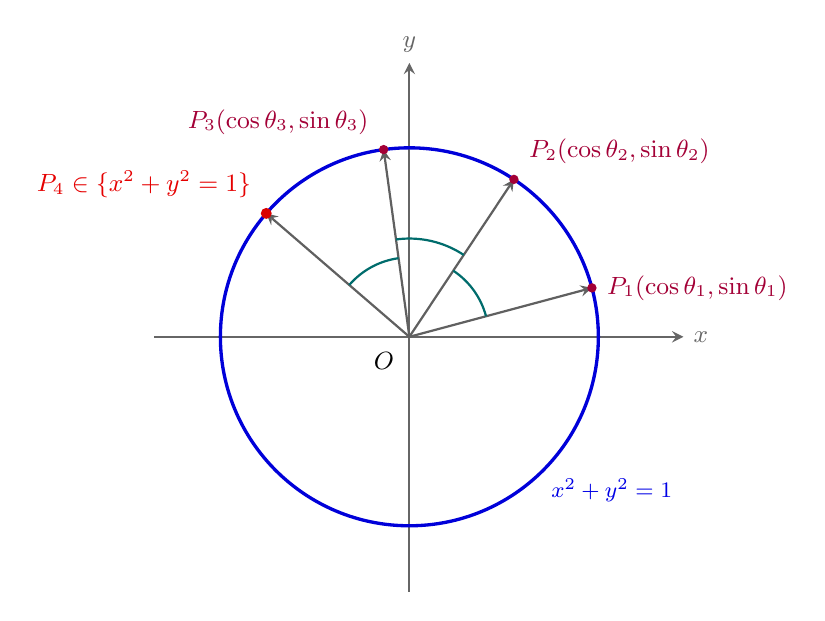
\begin{tikzpicture}[scale=2.4, >=stealth, every node/.style={font=\small}]

    % --- 1. 定数・厳密パラメータ ---
    % cos(delta) = 3/4 = 0.75 => delta ≈ 41.41°
    % theta_1 = 15° と設定
    \def\angDelta{41.4096}
    \def\angOne{15}
    \pgfmathsetmacro{\angTwo}{\angOne + \angDelta}         % ≈ 56.41°
    \pgfmathsetmacro{\angThree}{\angTwo + \angDelta}       % ≈ 97.82°
    \pgfmathsetmacro{\angFour}{\angThree + \angDelta}      % ≈ 139.23°

    \coordinate (O)  at (0, 0);
    \coordinate (P1) at ({\angOne}:1.0);
    \coordinate (P2) at ({\angTwo}:1.0);
    \coordinate (P3) at ({\angThree}:1.0);
    \coordinate (P4) at ({\angFour}:1.0);

    % --- 2. 座標軸 ---
    \draw[->, thick, gray!80!black] (-1.35, 0) -- (1.45, 0) node[right] {$x$};
    \draw[->, thick, gray!80!black] (0, -1.35) -- (0, 1.45) node[above] {$y$};
    \node[below left=2pt] at (O) {$O$};

    % --- 3. 単位円 x^2 + y^2 = 1 ---
    \draw[very thick, blue!85!black] (O) circle (1.0);
    \node[blue!90!black, font=\footnotesize\bfseries, below right] at (0.7, -0.7) {$x^2 + y^2 = 1$};

    % --- 4. 動径ベクトル OP_k ---
    \draw[->, thick, gray!75!black] (O) -- (P1);
    \draw[->, thick, gray!75!black] (O) -- (P2);
    \draw[->, thick, gray!75!black] (O) -- (P3);
    \draw[->, thick, gray!75!black] (O) -- (P4);

    % --- 5. 点プロットとラベル ---
    \node[circle, fill=purple!85!black, inner sep=1.2pt] at (P1) {}; \node[purple!85!black, right=2pt] at (P1) {$P_1(\cos\theta_1, \sin\theta_1)$};
    \node[circle, fill=purple!85!black, inner sep=1.2pt] at (P2) {}; \node[purple!85!black, above right=2pt] at (P2) {$P_2(\cos\theta_2, \sin\theta_2)$};
    \node[circle, fill=purple!85!black, inner sep=1.2pt] at (P3) {}; \node[purple!85!black, above left=2pt] at (P3) {$P_3(\cos\theta_3, \sin\theta_3)$};
    \node[circle, fill=red!85!black, inner sep=1.4pt] at (P4) {}; \node[above left=2pt, red!90!black] at (P4) {$P_4 \in \{x^2+y^2=1\}$};

    % --- 6. 隣り合う動径のなす角 delta の表示 ---
    % P1 と P2 の間の角
    \draw[thick, teal!85!black] (\angOne:0.42) arc (\angOne:\angTwo:0.42);
    % P2 と P3 の間の角
    \draw[thick, teal!85!black] (\angTwo:0.52) arc (\angTwo:\angThree:0.52);
    % P3 と P4 の間の角
    \draw[thick, teal!85!black] (\angThree:0.42) arc (\angThree:\angFour:0.42);

  \end{tikzpicture}
  \caption{単位円 $x^2+y^2=1$ 上の点列 $P_1, P_2, P_3, P_4$ と角間隔}
  \label{fig:unit_circle_pk_sequence}
\end{figure}

題意より$k=1,2,3$に対して$P_k(\cos\theta_k, \sin\theta_k)$ ($0 \le \theta_k < 2\pi$) とおく．\cref{eq:1}で$n=2$として
\begin{align}
  \begin{pmatrix} \cos\theta_3 \\ \sin\theta_3
  \end{pmatrix} = \dfrac{3}{2}
  \begin{pmatrix} \cos\theta_2 \\ \sin\theta_2
  \end{pmatrix} -
  \begin{pmatrix} \cos\theta_1 \\ \sin\theta_1
  \end{pmatrix} \label{eq:4}
\end{align}
だから，$\cos^3\theta_3+\sin^3\theta_3=1$に代入して
\begin{align}
  \left(\dfrac{3}{2}\cos\theta_2 - \cos\theta_1\right)^2 + \left(\dfrac{3}{2}\sin\theta_2 - \sin\theta_1\right)^2 &= 1 \\
  \dfrac{9}{4} - 3\cos(\theta_2 - \theta_1) &= 0 \\
  \cos(\theta_2 - \theta_1) &= \dfrac{3}{4} \label{eq:5}
\end{align}
である．

次に\cref{eq:1}で$n=3$とすると，
\begin{align}
  \overrightarrow{OP_4}
  &= \dfrac{3}{2}
  \begin{pmatrix} \dfrac{3}{2}\cos\theta_2 - \cos\theta_1 \\ \dfrac{3}{2}\sin\theta_2 - \sin\theta_1
  \end{pmatrix} -
  \begin{pmatrix} \cos\theta_2 \\ \sin\theta_2
  \end{pmatrix} \\
  &=
  \begin{pmatrix} \dfrac{5}{4}\cos\theta_2 - \dfrac{3}{2}\cos\theta_1 \\ \dfrac{5}{4}\sin\theta_2 - \dfrac{3}{2}\sin\theta_1
  \end{pmatrix}
\end{align}
である．ここで$|\overrightarrow{OP_4}|$を計算すると，
\begin{align}
  |\overrightarrow{OP_4}|^2
  &= \dfrac{25}{16} + \dfrac{9}{4} - \dfrac{15}{4}\cos(\theta_2 - \theta_1) \\
  &= \dfrac{25+36-45}{16} \quad (\because \text{\cref{eq:5}}) \\
  &= 1
\end{align}
となり，たしかに$P_4$も$x^2+y^2=1$上にある．

\end{document}
